% DO NOT COMPILE THIS FILE DIRECTLY!
% This is included by the other .tex files.

\begin{frame}[t,plain]
\titlepage
\end{frame}

\begin{frame}
    \frametitle{MISP \& STIX}
    \begin{itemize}
        \item \textbf{Built-in integration}
        \begin{itemize}
            \item Available from the UI
            \item Accessible via restSearch
        \end{itemize}
        \item []
        \item Export \& Import features
        \begin{itemize}
            \item Export MISP data collections
            \item Import STIX files
        \end{itemize}
        \item []
        \item Supported version
        \begin{itemize}
            \item STIX 1.1.1 \& 1.2
            \item STIX 2.0 \& 2.1
        \end{itemize}
    \end{itemize}
\end{frame}

\begin{frame}
    \frametitle{misp-stix - Key features}
    \begin{itemize}
        \item MISP $\Longleftrightarrow$ STIX conversion
        \begin{itemize}
            \item Used by MISP core to handle the conversion ability
            \item Preserve as much content \& context as possible
        \end{itemize}
        \item Support all the STIX versions
        \begin{itemize}
            \item \textbf{STIX 2.1 Support}
            \item 1.1.1, 1.2, 2.0 Support enhanced
        \end{itemize}
        \item []
        \item \textbf{Mapping documentation}\footnote{https://github.com/misp/misp-stix/tree/main/documentation\#readme}
        \item Package available on PyPI\footnote{https://pypi.org/project/misp-stix/}
    \end{itemize}
\end{frame}

\begin{frame}
    \frametitle{Handling the conversion with a python library}
    \begin{itemize}
        \item Integration in python code
        \begin{itemize}
            \item Automation made easier by a close coupling with PyMISP
            \begin{itemize}
                \item Export content from MISP
            \end{itemize}
        \end{itemize}
    \end{itemize}
    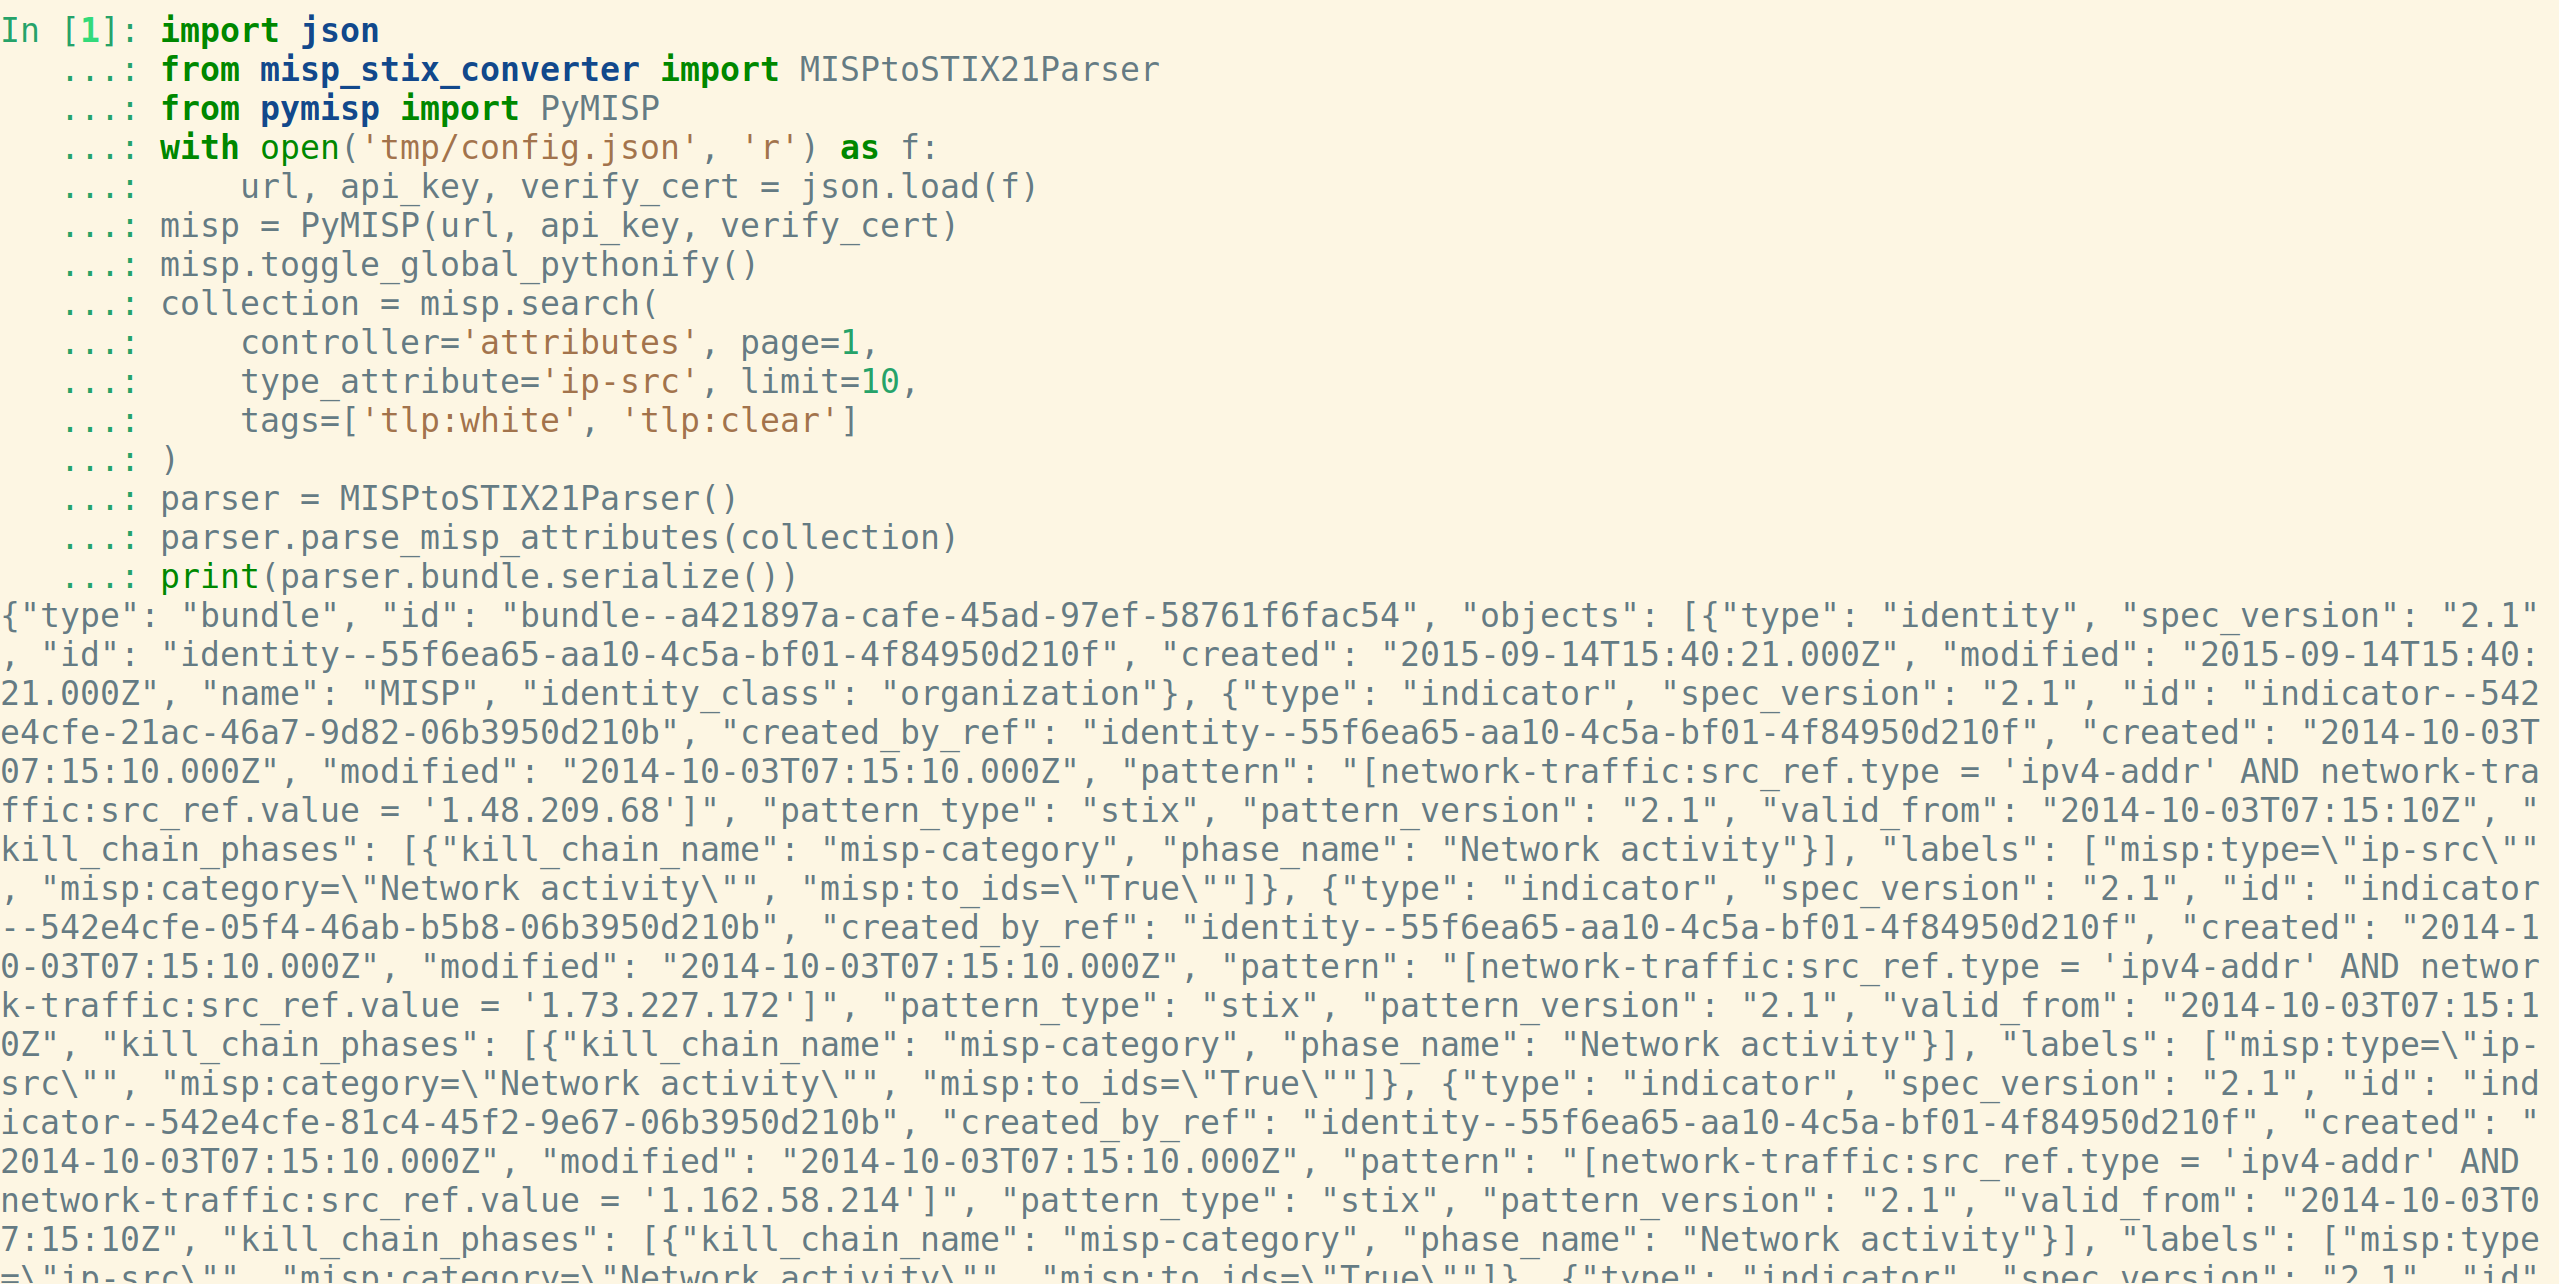
\includegraphics[scale=0.15]{images/PyMISPrestSearchMISP.png}
\end{frame}

\begin{frame}
    \frametitle{Handling the conversion with a python library}
    \begin{itemize}
        \item Integration in python code
        \begin{itemize}
            \item Automation made easier by a close coupling with PyMISP
            \begin{itemize}
                \item Export content from MISP
                \item Using the STIX return format directly
            \end{itemize}
        \end{itemize}
    \end{itemize}
    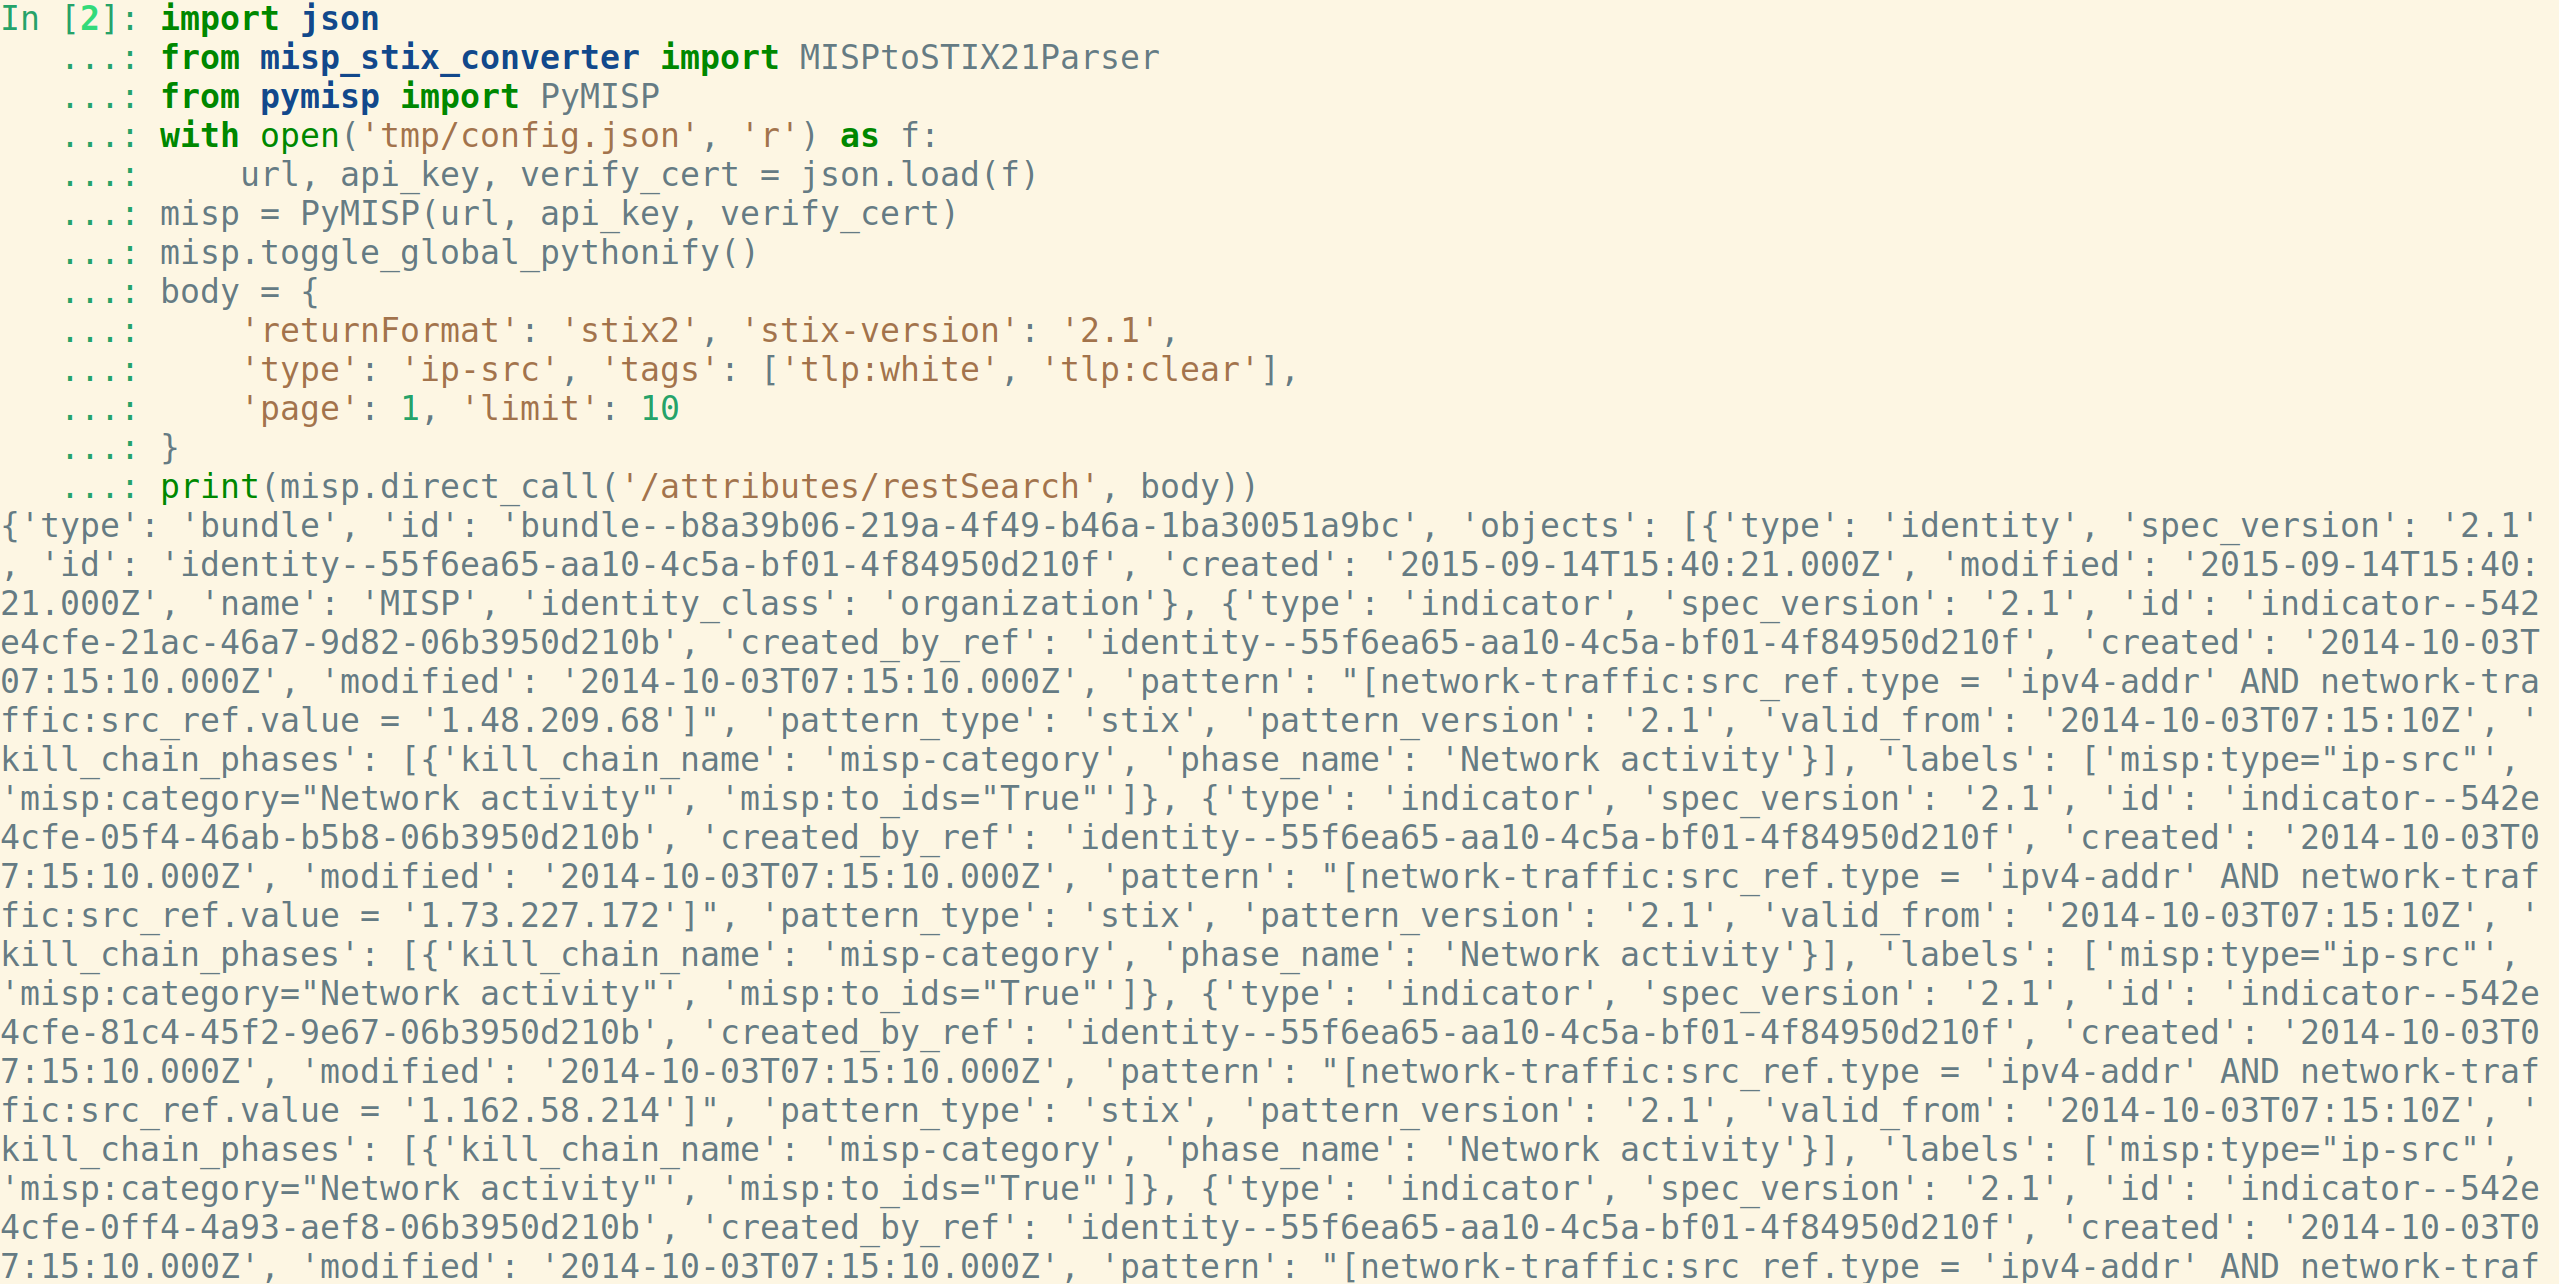
\includegraphics[scale=0.15]{images/PyMISPrestSearchSTIX.png}
\end{frame}

\begin{frame}
    \frametitle{Handling the conversion with a python library}
    \begin{itemize}
        \item Integration in python code
        \begin{itemize}
            \item Automation made easier by a close coupling with PyMISP
            \begin{itemize}
                \item Converting STIX content and adding the resulting Event
                \begin{center}
                    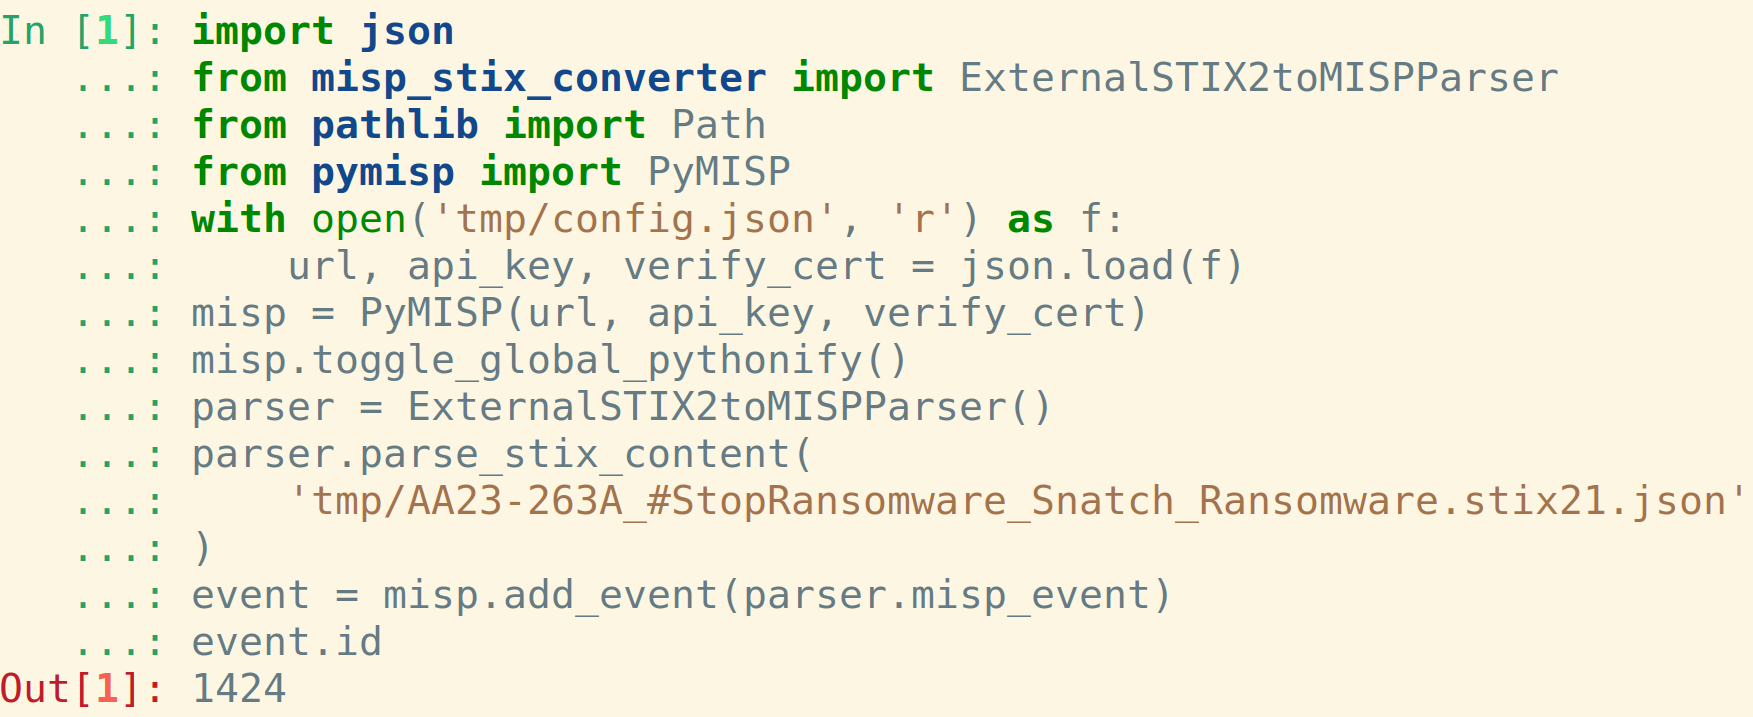
\includegraphics[scale=0.15]{images/PyMISPaddEvent.png}
                \end{center}
                \item Using the API endpoint directly
                \begin{center}
                    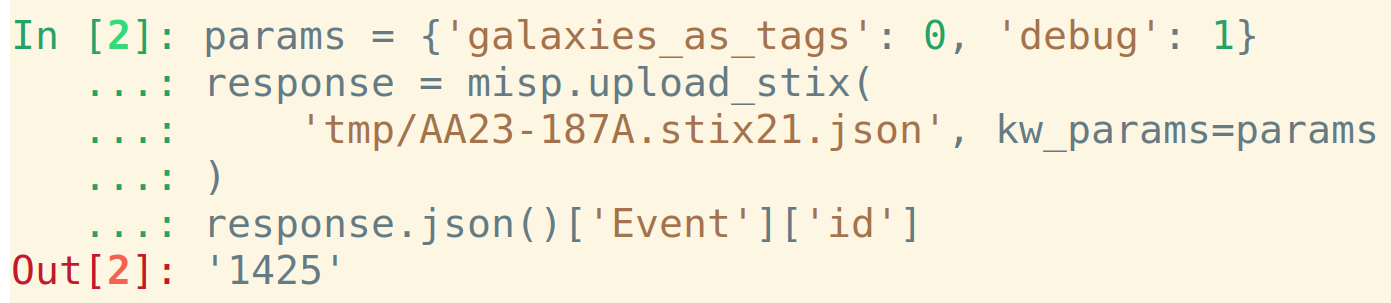
\includegraphics[scale=0.15]{images/PyMISPuploadSTIX.png}
                \end{center}
            \end{itemize}
        \end{itemize}
    \end{itemize}
\end{frame}

\begin{frame}
    \frametitle{Handling the conversion with a python library}
    \begin{itemize}
        \item Addressing the limitations of a MISP built-in integration
        \begin{itemize}
            \item Export \& import features available as a command-line application
        \end{itemize}
    \end{itemize}
    \centering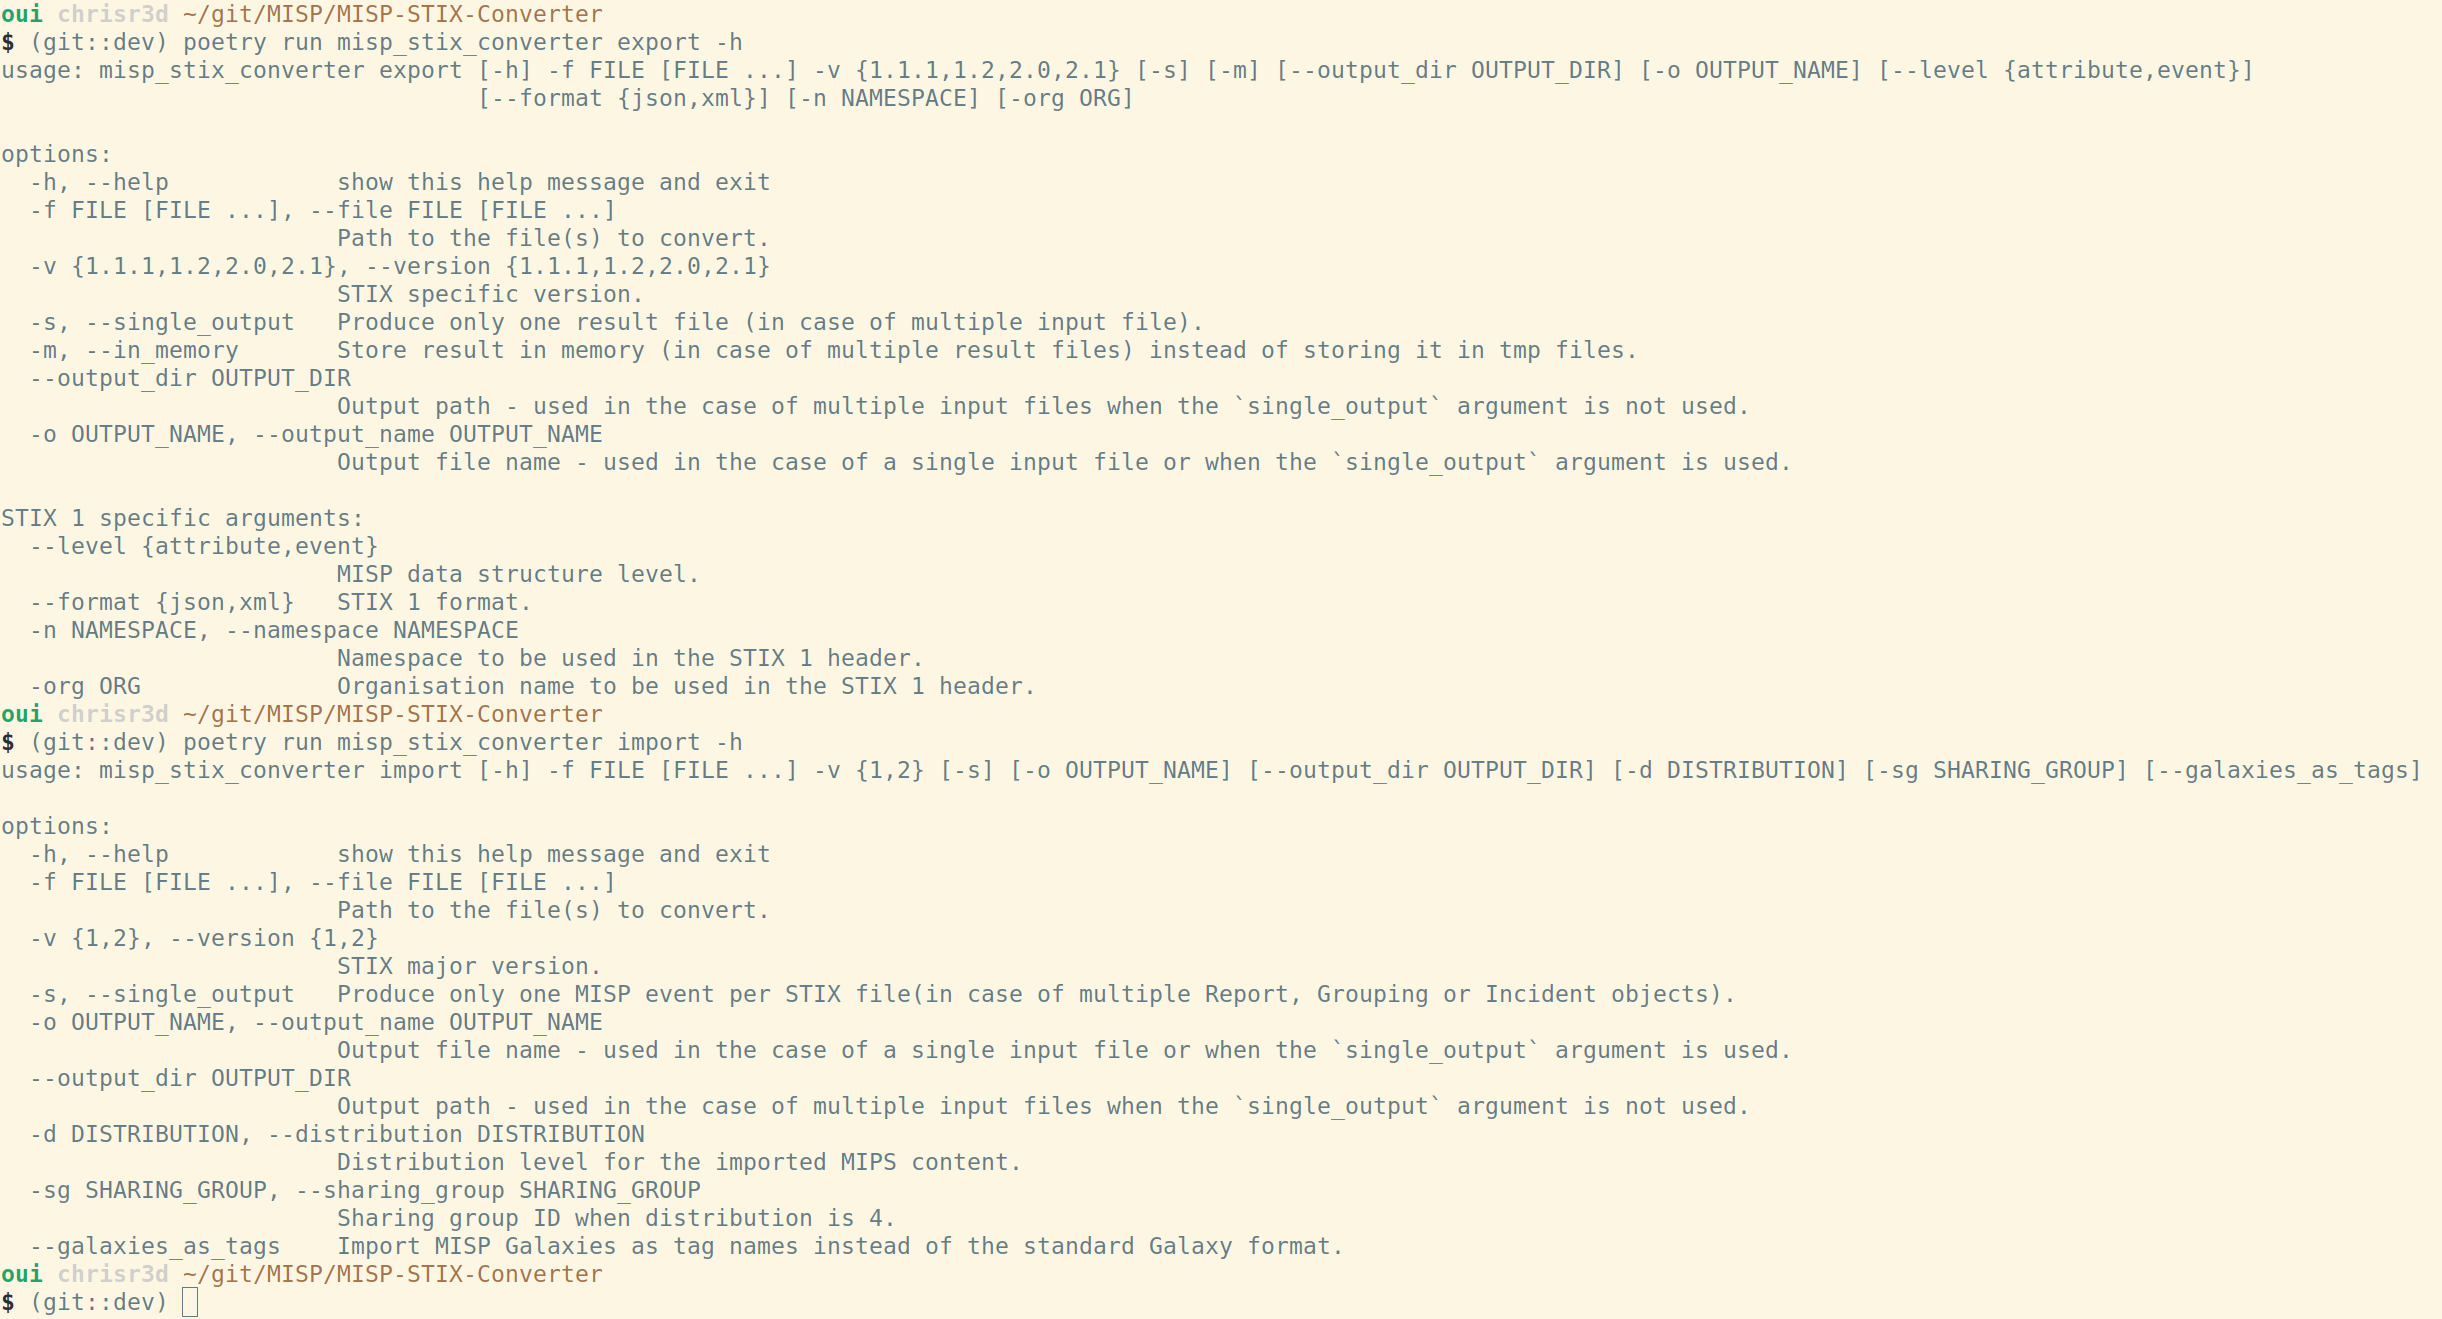
\includegraphics[scale=0.14]{images/command_line_help.png}
\end{frame}

\begin{frame}
    \frametitle{Handling the conversion with a python library}
    \begin{itemize}
        \item Addressing the limitations of a MISP built-in integration
        \begin{itemize}
            \item Export \& import features available as a command-line application
        \end{itemize}
    \end{itemize}
    \centering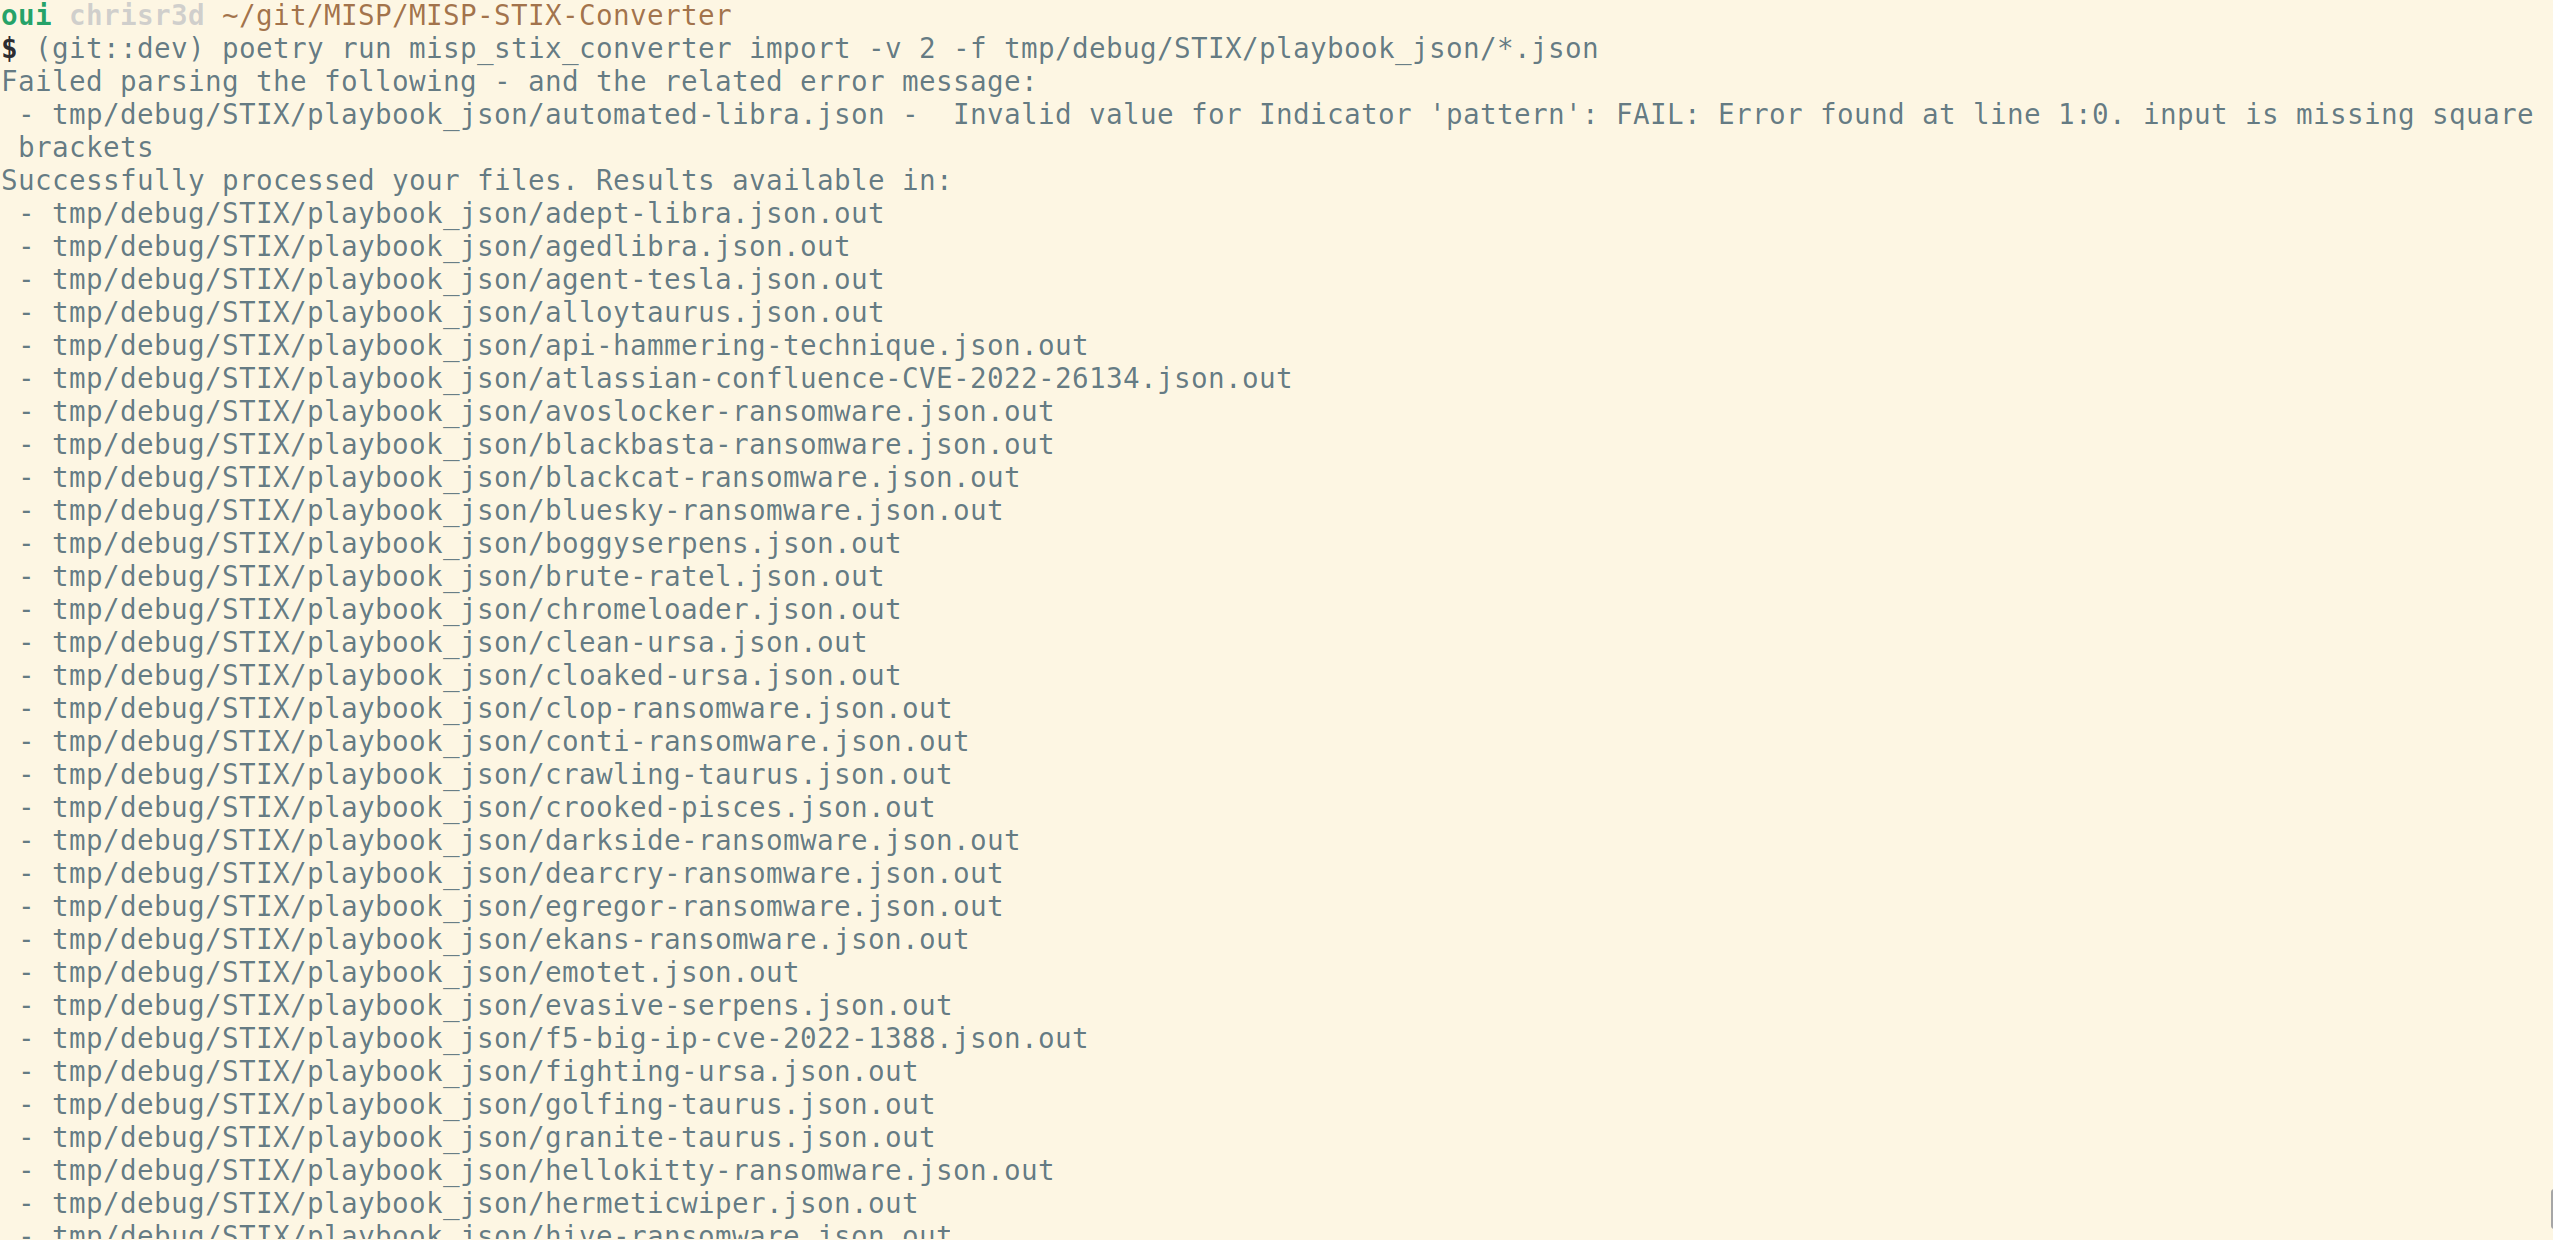
\includegraphics[scale=0.14]{images/stix_import_results.png}
\end{frame}

\begin{frame}
    \frametitle{Continuous Work in Progress \& Improvement}
    \begin{itemize}
        \item {\bf Improve the import feature}
        \begin{itemize}
            \item Handle different content design from different sources
            \item Support of existing STIX objects libraries\footnote{https://github.com/mitre/cti}
            \item Support custom STIX format
            \item \textbf{Handle validation issues}
        \end{itemize}
        \item Continuous MISP $\Longleftrightarrow$ STIX mapping improvement
        \item More tests to avoid edge case issues
        \item []
        \item Participating in Oasis CTI TC
    \end{itemize}
    \centering
\includegraphics[scale=0.2]{images/oasis.png}
\end{frame}

\begin{frame}
    \frametitle{How to report bugs/issues}
    \begin{itemize}
        \item Github issues
        \begin{itemize}
            \item {\bf https://github.com/MISP/misp-stix/issues}
            \item https://github.com/MISP/MISP/issues
        \end{itemize}
        \item []
        \item Please provide details
        \begin{itemize}
            \item How did the issue happen
            \item {\bf Recommendation}: provide samples
        \end{itemize}
        \item[]
        \item Any feedback welcome
    \end{itemize}
\end{frame}

\begin{frame}
    \frametitle{To get in touch with us}
    \begin{itemize}
        \item \url{https://github.com/MISP/misp-stix}
        \item \url{https://github.com/MISP/misp-stix/tree/main/documentation}
        \item []
        \item \url{https://github.com/MISP}
        \item \url{https://www.misp-project.org/}
        \item \url{https://twitter.com/MISPProject}
        \item \url{https://twitter.com/chrisred_68}
    \end{itemize}
\end{frame}
